\documentclass[   
state        = Poster,                       % (Report | Poster    | Thesis)
lang         = EN,                           % (DE     | EN) 
dept         = MECH,                         % (MECH   | SBT)
bib-active   = true,                         % (true   | false)
bib-style    = ieee,                         % (ieee)
]{mcidoc}

% CUSTOM COMMANDS -----------------------------------------------------------------------------
%       
% Please enter any custom command/packages you require here for easy tracking 

% For example, bibliography setting are added. Bibtex is the standard but if you prefer
% there are other options on the market such as biber. Style has been chosen as IEEE but if 
% are from another discipline, please feel free to change it.




\bibliography{references.bib}  % Here we add our file where we store our references.
%      
% ---------------------------------------------------------------------------------------------

% DOCUMENT PARAMETERS -------------------------------------------------------------------------

\Title{%
  On the Study of Different Rotor Geometry Configuration for use in High-Speed
  Induction Motors
}% 

\Authors{%
  Alvin McCollough
}%

\Affiliations{%
  MCI, Innsbruck, Austria
}%

\begin{document} % ############################################################################

\MakeTitlePage

\begin{columns}
	\column{0.39}  
	\block{Defining Speed}{ 
		In recent years, improvements in manufacturing, transportation and process industry
		technologies bring about an increase in optimal operation speed in drive systems. In this
		respect, recently developed high speed gear-less or direct-drive electrical drives have seen an
		increase in interest based on the reduction in the total structural volume of the drive
		system. Due to the significant development of cost-effective, fast switching and compact
		variable frequency drives technology, wide speed range operations of different type AC motors
		has become feasible. The speed definition of an induction motor can be seen in Eq.\ \ref{eq:speed}

		\begin{equation}  \label{eq:speed}
			n = \frac{120 f}{p},
		\end{equation}

		In literature, there are several descriptions for the term "high-speed".  As a mechanical
		engineer, peripheral speed over \SI{150}{\meter\per\second} is considered to be high speed
		\cite{gieras2011performance}. From the motor manufacturer's point of view, a two-pole machine
		which is supplied higher than 50 to \SI{60}{\hertz}, can be considered as a high-speed machine.
		However, the most important point of view for the high-speed term is explained by development
		at power electronics. Nowadays, up to few hundreds hertz frequencies can be produced by
		variable frequency drives. However, voltage qualities of these are not satisfactory due to
		limited switching frequency of high-power IGBT technology. Thus, high-speed levels might be
		calculated for frequencies in the range of 100 to \SI{400}{\hertz} are considered to be
		high-frequencies \cite{pyrhonen1991high}.  Owing to brush and commutator structure causing mechanical and
		electrical problems, DC drives are not allowed to be used for high-speed applications. In
		addition to the aforementioned statement, the structure is not appropriate for large
		centrifugal forces.  Nevertheless, as high-speed drive applications, there are different type
		of AC motor concepts proposed in literature
		\cite{gieras2011performance, pyrhonen1991high, lahteenmaki2002design, saari1998thermal}:
		Laminated/solid induction, permanent
		magnet synchronous and switched reluctance synchronous motors.
	}
	~
	\column{0.59}
	\block{Comparison}{
		It is due to remarkable improvements of power electronics, frequency inverters and AC
		variable-speed drives, which allows a wider use of applications of solid-rotor induction motor
		(SRIM). SRIM's are used in drive application ranging from a few kW's to 10 MW's. Fans,
		compressors, pumps, gas turbines, sewing machines, space and aeronautics, auxiliary motors for
		starting turbo-alternators, eddy current brakes, two-phase servomotors are a few examples of its
		areas.

		Below are the advantages of SRIM compared to CRIM:

		\begin{itemize}[itemsep=0pt]
			\item Structural and Mechanical integrity, Rigiditiy, Reliability and Strength of
			      Material
			\item High thermal properties
			\item High speed in high power applications (high moment density)
			\item Low noise and vibrations in high speed applications
			\item Simple to protect against aggressive chemicals
			\item Ease of Manufacturing
			\item Low level of noise and vibrations (If the rotor has no slots)
			\item Linearity of torque-speed characteristics throughout the entire speed range
			\item The possibility of obtaining steady-state stability.
		\end{itemize}
	}
    ~
	\block{A Figure}{
		In 1950s, Solid-Rotor topologies for induction machines operating at high speeds
		have gained a lot of interest. From its inception to 1970s, various scientists and engineers
		have contributed to the development and the theory of solid rotor construction, where significant
		interest was seen the 1990s for using solid rotor structure for high speed applications.

		\begin{tikzfigure}
			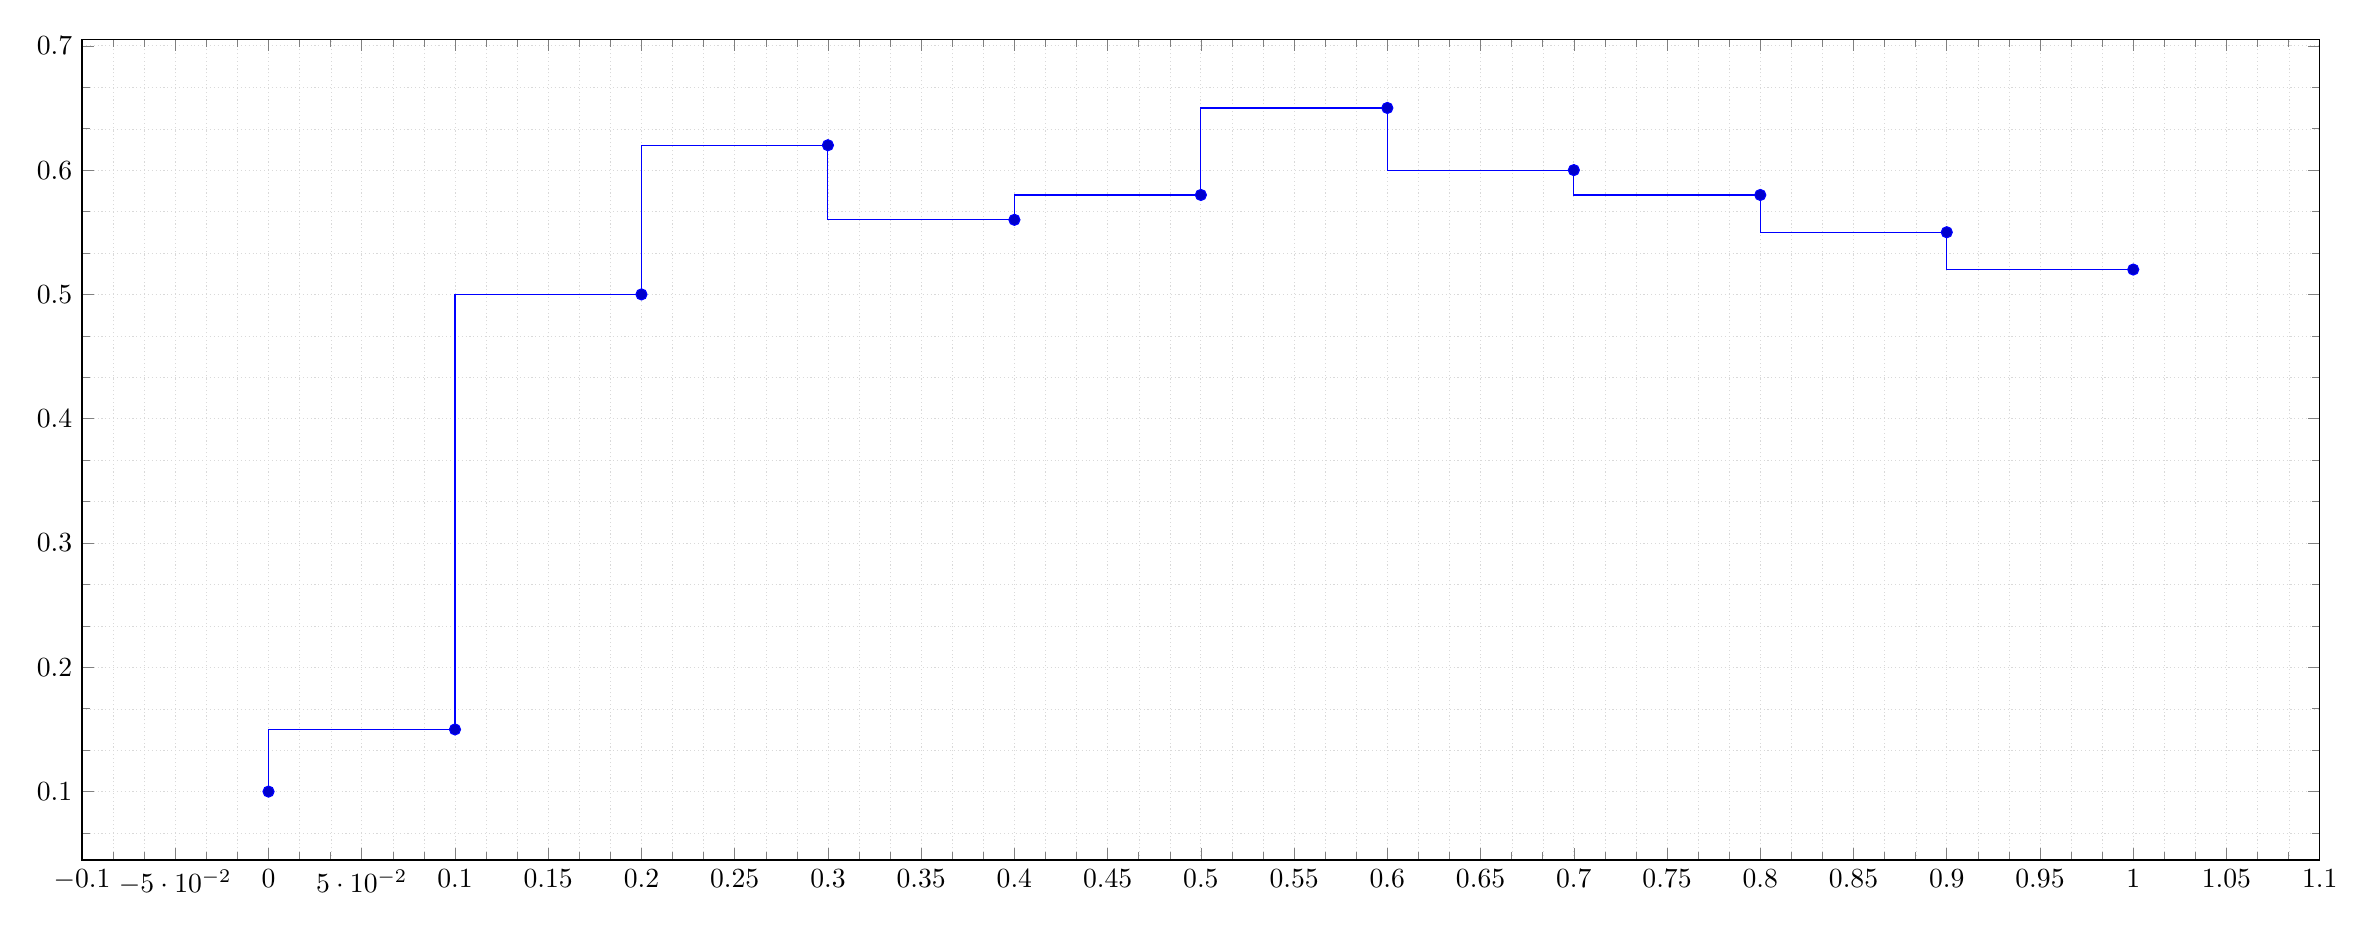
\begin{tikzpicture}
				\begin{axis}[width=30cm, height=12cm,
						minor tick num   = 2,
						grid             = both,	% have a grid that is bitchin
						% GRID OPTIONS
						minor grid style = {
								densely dotted,
								line width = 0.1,
								gray!30
							},
						major grid style={
								densely dotted,
								line width = 0.3,
								gray!30
							}]
					\addplot+ [
						const plot mark right,
					] coordinates {
							(0,0.1)    (0.1,0.15)  (0.2,0.5)   (0.3,0.62)
							(0.4,0.56) (0.5,0.58)  (0.6,0.65)  (0.7,0.6)
							(0.8,0.58) (0.9,0.55)  (1,0.52)
						};
				\end{axis}
			\end{tikzpicture}
		\end{tikzfigure}
	}
\end{columns}

\begin{columns}
	\column{0.98}
	\block{Another Block}{
		In this report for Drive Technologies, the high-speed performance of the four
		different types of rotors are investigated and compared using finite element analysis:
		cage, smooth solid, axially slitted, coated is designed using a finite-element
		analysis (FEA). All rotors are designed with similar geometries and construction parameters
		to minimise the effect of unwanted effects.

		The number of turns per stator slot is selected so as to obtain the
		same stator current in rated operation. All four motors were analyzed using FEA
		tools for 20 different speeds in order to obtain the combined torque-speed
		characteristics. To illustrate visually the differences in the distributions of the
		magnetic flux and the eddy current the results for 11300 rpm are presented and the
		core loss, the total loss and the efficiency for the specific speed are compared for all
		the motors. The designed four motors will be also compared for winding currents,
		induced voltages, flux linkages, electromagnetic torque, copper losses, iron losses,
		solid rotor losses and efficiency.
      }
      \block{References}{
        \printbibliography[heading=none]
        }
\end{columns}

\end{document} % \(^.^)/
